% <===================================================================
% <======================					==========================
% <======================	USEPACKAGES	==========================
% <======================					==========================
% <===================================================================

\documentclass{article}
\usepackage{xcolor}
\usepackage[utf8]{inputenc}
\usepackage{float}
\usepackage{textmerg} 
\usepackage{wrapfig}
\usepackage{tikz}
\usetikzlibrary{shapes.geometric, calc}
\usetikzlibrary{calc,shadows,shadows.blur}
\usepackage{tabularx,booktabs} 
\usepackage[space]{grffile}
\usepackage[sfdefault]{ClearSans}
\usepackage[margin=0.2in]{geometry}

 
% <===================================================================
% <======================					==========================
% <======================	New Commands	==========================
% <======================					==========================
% <===================================================================


\newcommand{\makeprofile}{
	\begin{tikzpicture}[remember picture,overlay]
   		\node [rectangle, fill=lightgray, anchor=north east, minimum width=8cm, minimum height=\paperheight+5cm] (box) at (21.5cm,5cm){};
	\end{tikzpicture}}

\newcommand\Slider[2]{
    \tikz[baseline=-0.1cm]{
        \coordinate (start) at (0,0);
        \coordinate (end) at (#1,0);
        \coordinate (mark) at ($(start)!#2!(end)$);
        \useasboundingbox (start|- 0,-.25) rectangle (end|- 0, .25);
        \draw[line width=0.4mm, line cap=round, white] 
             (start) -- (mark) edge[white] (end);
        \node[fill=custom, draw=custom, very thin,
            blur shadow={shadow xshift=0pt, shadow opacity=20, shadow yshift=-0.9mm,
                         shadow blur steps=6, shadow blur radius=0.3mm},
            circle, minimum size=0.25cm, inner sep=0pt] at (mark) {};
    }
}

\newcommand\score[2]{%
  \pgfmathsetmacro\pgfxa{#1 + 1}%
  \tikzstyle{scorestars}=[star, star points=5, star point ratio=2.25, inner sep=0.15em, anchor=outer point 3]%
  \begin{tikzpicture}[baseline]
    \foreach \i in {1, ..., #2} {
      \pgfmathparse{\i<=#1 ? "custom" : "gray"}
      \edef\starcolor{\pgfmathresult}
      \draw (\i*1em, 0) node[name=star\i, scorestars, fill=\starcolor]  {};
    }
    \pgfmathparse{#1>int(#1) ? int(#1+1) : 0}
    \let\partstar=\pgfmathresult
    \ifnum\partstar>0
      \pgfmathsetmacro\starpart{#1-(int(#1)}
      \path [clip] ($(star\partstar.outer point 3)!(star\partstar.outer point 2)!(star\partstar.outer point 4)$) rectangle 
      ($(star\partstar.outer point 2 |- star\partstar.outer point 1)!\starpart!(star\partstar.outer point 1 -| star\partstar.outer point 5)$);
      \fill (\partstar*1em, 0) node[scorestars, fill=custom]  {};
    \fi
  \end{tikzpicture}%
}


% <===================================================================
% <======================					==========================
% <======================	Page/Color Style 	==========================
% <======================					==========================
% <===================================================================
 
 \begin{document}
 


 \begin{titlepage}
 	\raggedleft % Right align the title page
	
	\rule{1pt}{\textheight} % Vertical line
	\hspace{0.05\textwidth} % Whitespace between the vertical line and title page text
	\parbox[b]{0.75\textwidth}{ % Paragraph box for holding the title page text, adjust the width to move the title page left or right on the page
		
		{\Huge\bfseries A Wine Portfolio \\[0.5\baselineskip]}  % Title
		{\large\textit{A Series of automated Factsheets based on a small wine database}}\\[4\baselineskip] % Subtitle or further description
		{\Large\textsc{Jonas \& Judith}} % Author name, lower case for consistent small caps
		
		\vspace{0.5\textheight} % Whitespace between the title block and the publisher
		
		{\noindent in vino veritas }\\[\baselineskip] % Publisher and logo
	}

\end{titlepage}
\newpage
\section{Overview of Wine Universe}
\newpage

\begin{figure}[H]
    \vspace*{0.2cm}
    \makebox[\linewidth]{
        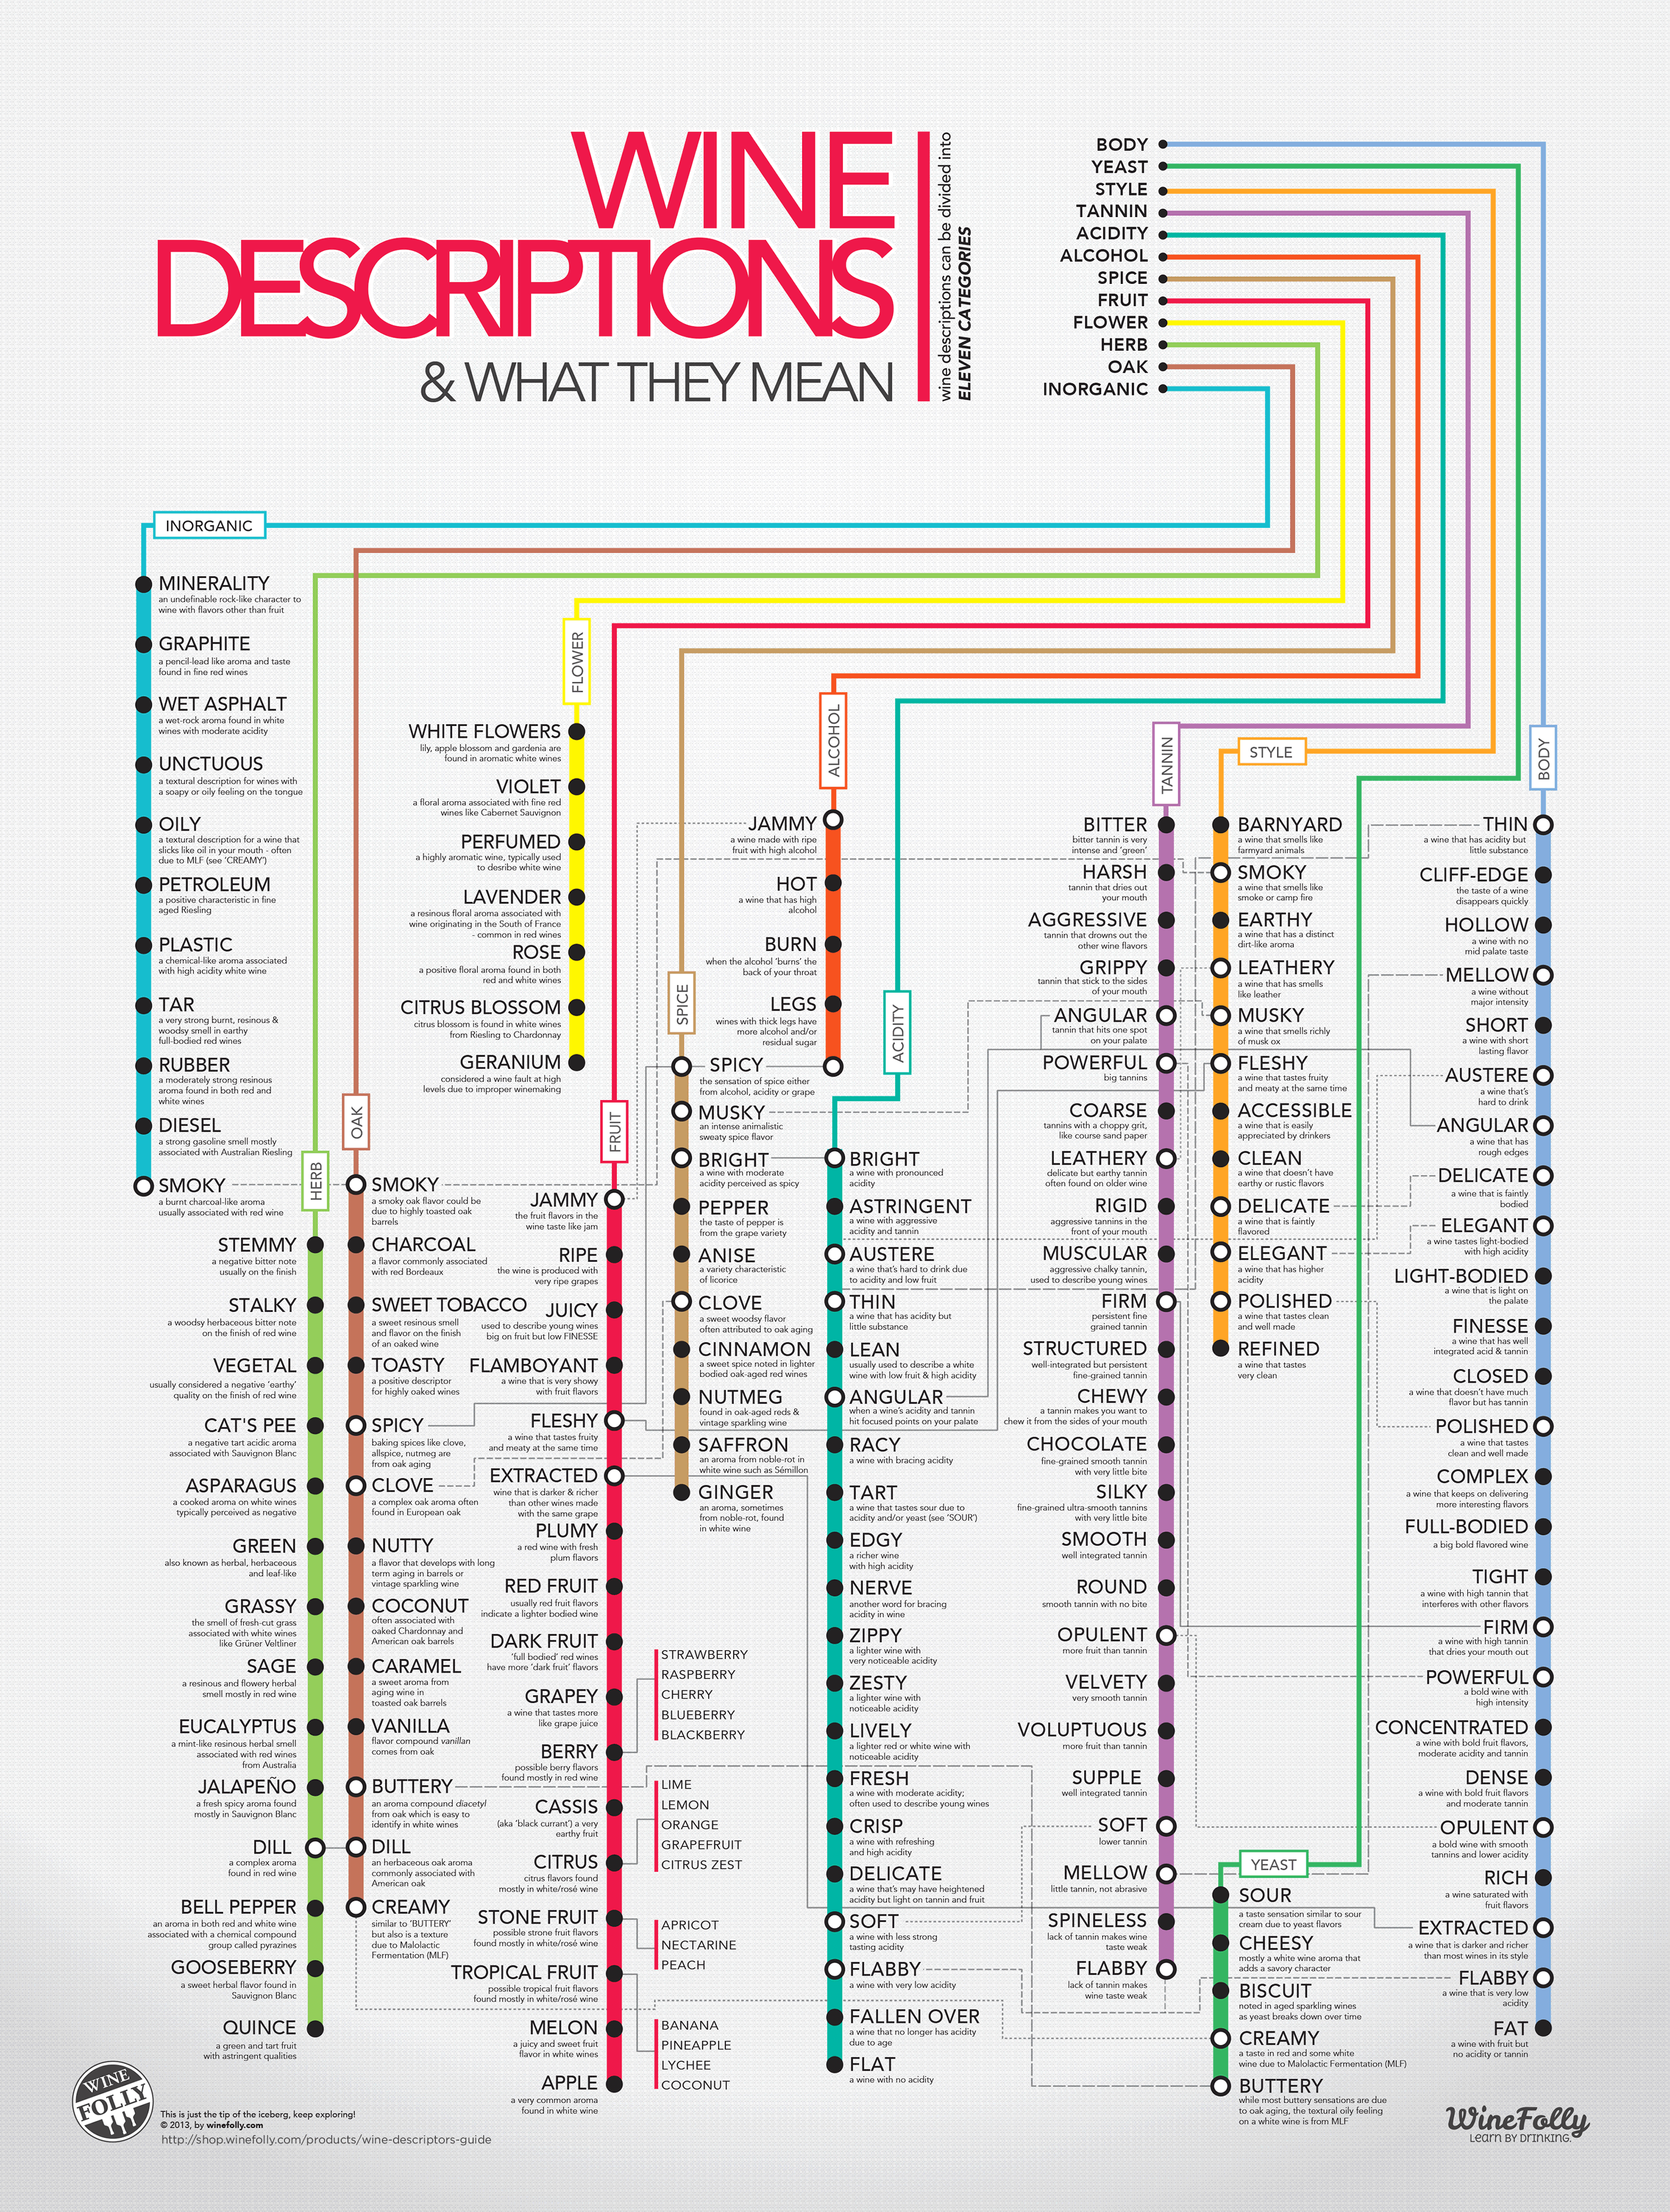
\includegraphics[width=\linewidth]{Pictures/Winedescription.png}
    }
\end{figure}

\newpage

\begin{figure}[H]
    \vspace*{0.6cm}
    \makebox[\linewidth]{
        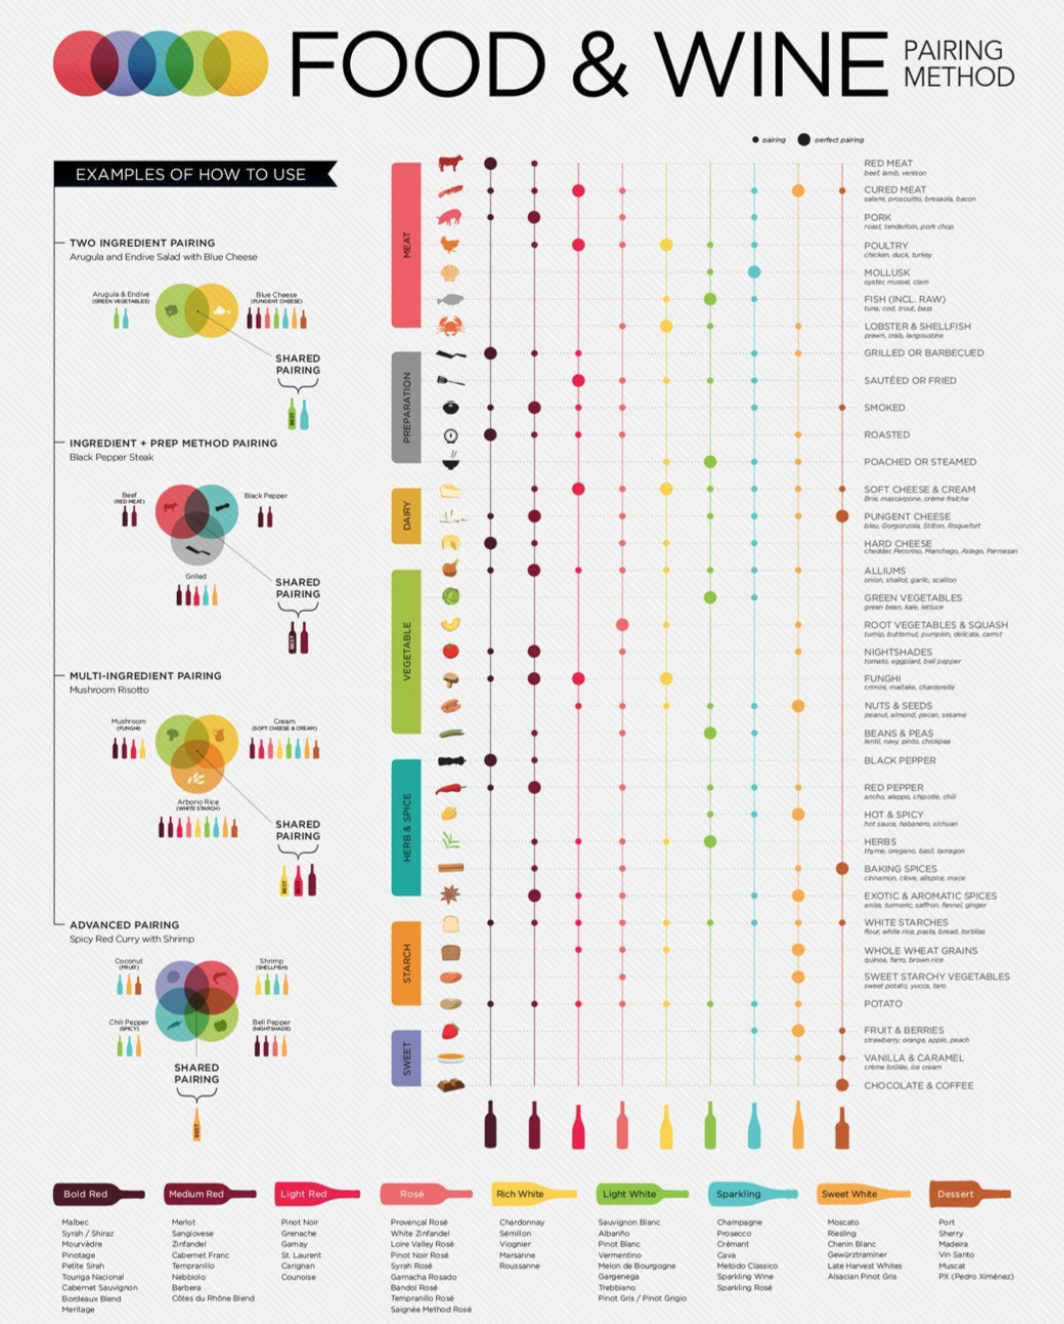
\includegraphics[width=\linewidth]{Pictures/FoodandWine.png}
    }
\end{figure}

\newpage

\begin{figure}[H]
    \vspace*{-0.3cm}
    \makebox[\linewidth]{
        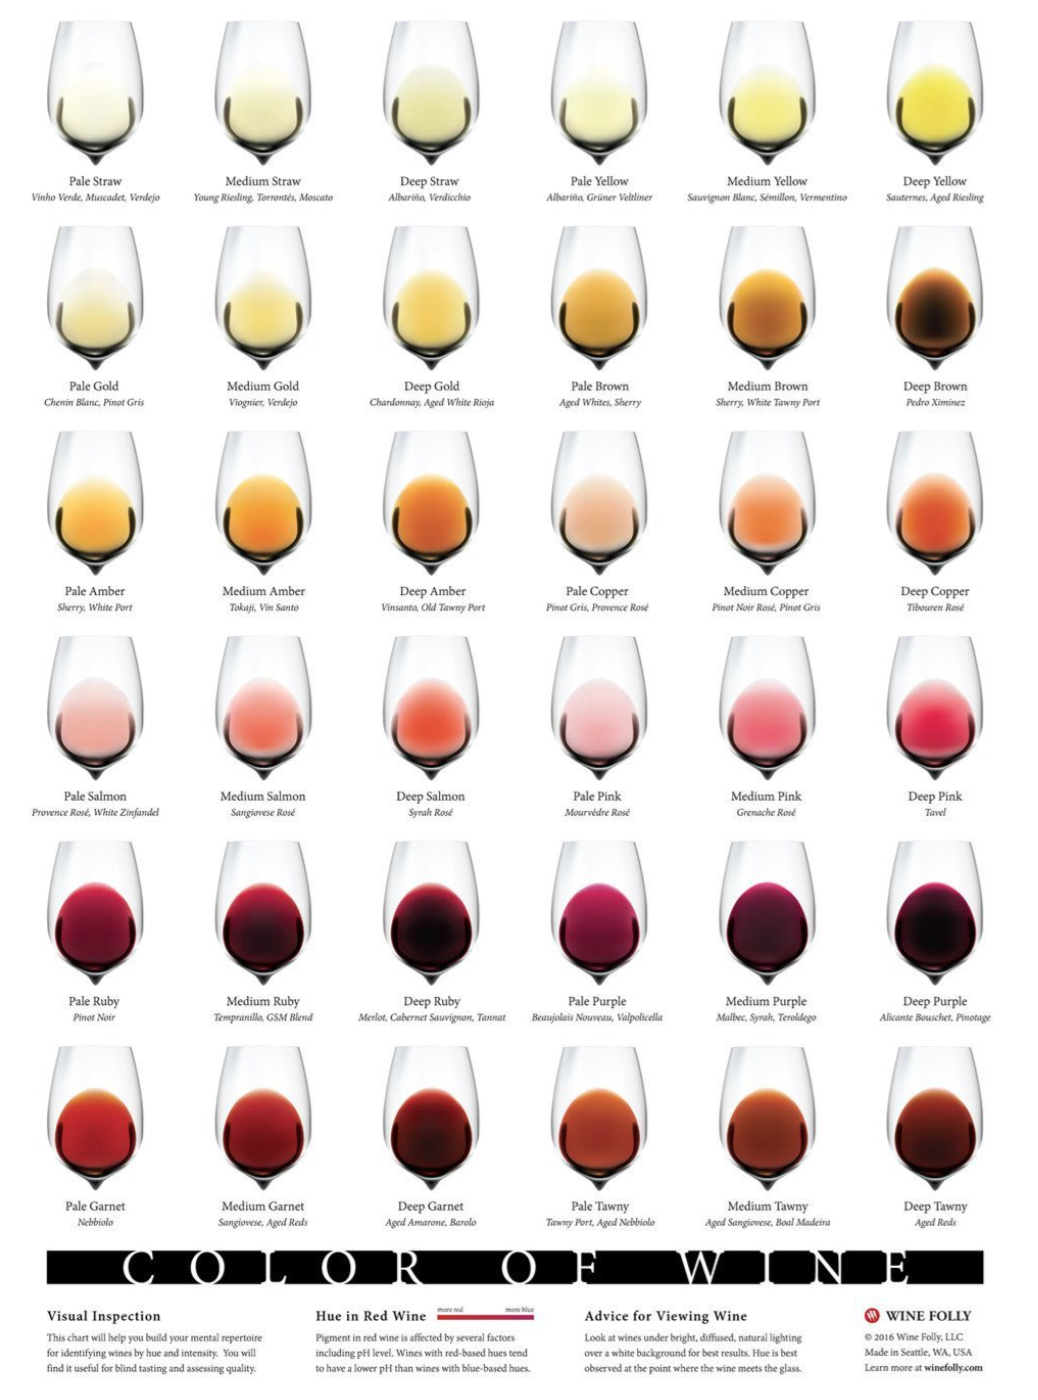
\includegraphics[width=\linewidth]{Pictures/Winecolor.png}
    }
\end{figure}

\newpage

\section{Factsheets based on our wine database }

\newpage

 
 \Fields{\Name\PictureID\Year\Rating\PriceRange\Winery\WineryDescription\Country\Region\Category\LighttoBold\SmoothtoTannic\DrytoSweet\SofttoAcidic\Catone\Cattwo\Grapes\WineStyle\WineStyleDescription\Alcohol\MainImpressionsA\MainImpressionsB\MainImpressionsC\FoodPairing\Notes\Color} 
 
 

 \Merge{data.dat}{
\newpage
\pagestyle{empty} 


\definecolor{custom}{HTML}{\Color}
%Spain: CF5300
%France: 003366
%Italy: 006400
%germany: 654321
%Austria: 8b0000

\makeprofile

% <===================================================================
% <======================					==========================
% <======================	Title/Rating/Price 	==========================
% <======================					==========================
% <===================================================================



\begin{minipage}{0.12\textwidth}
\includegraphics[height=5cm]{Pictures/\PictureID.png} 
\end{minipage}
\begin{minipage}{0.54\textwidth}
\begin{minipage}{0.9\textwidth}
 \raggedright
\Huge \textbf{\textcolor{custom}{\Winery }} \newline
 \textit{\textcolor{custom}{\Name}} \newline
 \large \includegraphics[width=0.5cm]{Pictures/\Country.png}  -- \large \Category  \ from \Region, \Country, Vintage \Year \LARGE
\end{minipage}
\end{minipage}
\begin{minipage}{0.25\textwidth}
\begin{tabularx}{\textwidth}{p{1.5cm}c}
\LARGE \textcolor{white}{ \Rating}  &  \Large{\score{\Rating}{5}}   \\[5ex]
\LARGE \textcolor{white}{ \$\$} &  \LARGE \textcolor{custom}{ \PriceRange}  \\[5ex]
\end{tabularx}
\end{minipage}
\newline \newline \newline

% <===================================================================
% <======================						======================
% <======================	Winery/Impression/Food 	======================
% <======================						======================
% <===================================================================

 \begin{minipage}[t]{0.66\textwidth}
\LARGE \textcolor{custom}{ \textbf{Winery: }\Winery} \newline
\small \begin{minipage}[t]{0.925\textwidth} 
\begin{wrapfigure}{r}{0.25\textwidth}
\vspace{-12pt}

\includegraphics[width=0.25\textwidth]{Pictures/\Region.png}
\vspace{-14pt}
\end{wrapfigure}
\vspace{10pt}
\WineryDescription \\
\end{minipage}
\end{minipage}
\begin{minipage}[t]{0.25\textwidth}
\LARGE  \textcolor{custom}{Main Impressions} \newline
 
\small \begin{tabularx}{\textwidth}{cl}
\textcolor{white}{$\bigcirc$}   & \MainImpressionsA  \\[4ex]
 \textcolor{white}{$\circ$}  &  \MainImpressionsB  \\[4ex]
 \textcolor{white}{$\cdot$}  &  \MainImpressionsC  \\[4ex]
\end{tabularx}  \newline
\vspace{5pt}

\LARGE  \textcolor{custom}{Food Pairing} \newline

\small \begin{tabularx}{\textwidth}{cl}
\includegraphics[width=0.5cm]{Pictures/Pairing.png}& \FoodPairing   \\
\end{tabularx}
\end{minipage}
\newline \newline \newline 


% <===================================================================
% <======================					==========================
% <======================	Style/Taste	 	==========================
% <======================					==========================
% <===================================================================



 \begin{minipage}[t]{0.66\textwidth}
\LARGE \textcolor{custom}{ \textbf{Wine Style:} \WineStyle}  \newline   
\small \begin{minipage}[t]{0.925\textwidth}
\vspace{10pt}
\WineStyleDescription \\
\end{minipage}
\end{minipage}
\begin{minipage}[t]{0.25\textwidth}
\LARGE  \textcolor{custom}{Taste Profile}\newline

\small \begin{tabular}{lll}
Light & \Slider{3.3cm}{\LighttoBold} & Bold \\
&  &  \\
\Catone & \Slider{3.3cm}{\SmoothtoTannic} & \Cattwo \\
&  &  \\
Dry & \Slider{3.3cm}{\DrytoSweet} & Sweet \\
&  &  \\
Soft & \Slider{3.3cm}{\SofttoAcidic} & Acidic \\
\end{tabular}
\end{minipage}
 \newline  \newline \newline 
 
 % <===================================================================
% <======================					==========================
% <======================	Notes/Essentials 	==========================
% <======================					==========================
% <===================================================================


 \begin{minipage}[t]{0.66\textwidth}
\LARGE \textcolor{custom}{ \textbf{Personal Notes:} Vintage \Year} \newline 
\small \begin{minipage}[t]{0.925\textwidth}
\vspace{10pt}
\Notes \\
\end{minipage}
\end{minipage}
\begin{minipage}[t]{0.25\textwidth}
\LARGE  \textcolor{custom}{Fundamentals} \newline 

\small \begin{tabularx}{\textwidth}{cl}

\includegraphics[width=0.38cm]{Pictures/Region.png} &  from \Region , \Country  \\[2ex]

\includegraphics[width=0.5cm]{Pictures/Winestyle.png}  &  \WineStyle  \\[2ex]

\includegraphics[width=0.5cm]{Pictures/Winery.png}  & \Winery  \\[2ex]

\includegraphics[width=0.5cm]{Pictures/Grapes.png} &  \Grapes  \\[2ex]

\includegraphics[width=0.5cm]{Pictures/Alc.png} &  \Alcohol \% \\[2ex]
\end{tabularx}
\end{minipage}

}
\section*{\textit{Fin}}

\newpage

\end{document}